1.3 և 1.4 պարագրաֆները նվիրված են լրիվ գրաֆների միջակայքային ներկումների ուսումնասիրությանը: Հայտնի է, որ լրիվ գրաֆը ունի միջակայքային ներկում այն և միայն այն դեպքում, երբ գագաթների քանակը զույգ է: Հայտնի է նաև, որ $w(K_{2n})=2n-1$: Քամալյանը ստացել է $W(K_{2n}) \geq 2n-1 + \left\lfloor \log_2(2n-1) \right\rfloor$ գնահատականը, որը հետագայում լավացվել է Պետրոսյանի կողմից\footnote{P.A. Petrosyan, Interval edge-colorings of complete graphs and n-dimensional cubes, Discrete Math. 310, 2010, pp. 1580-1587.}.
\begin{hide}
\begin{theorem}\cite{Kamalian1990}
Ցանկացած $n\in \mathbb{N}$ թվի համար $W(K_{2n}) \geq 2n-1 + \left\lfloor \log_2(2n-1) \right\rfloor$:
\end{theorem}
\begin{theorem}\cite{Petrosyan2010}\label{tPetrosyan3n2}
Ցանկացած $n\in \mathbb{N}$ թվի համար $W(K_{2n}) \geq 3n-2$:
\end{theorem}
\begin{theorem}\cite{Petrosyan2010}\label{tPetrosyan4n}
Ցանկացած $n\in \mathbb{N}$ թվի համար $W(K_{4n}) \geq 4n-1 + W(K_{2n})$:
\end{theorem}
\end{hide}
\begin{theorem}
\label{t2_complete_pq} Եթե $n=p2^{q}$, որտեղ $p$-ն կենտ է, իսկ $q \in \mathbb{Z}_{\geq 0}$, ապա
\begin{center}
$W\left(K_{2n}\right)\geq 4n-2-p-q$:
\end{center}
\end{theorem}

\begin{hide}
\begin{hypothesis}
\label{h1_complete_pq}
Եթե $n=p2^{q}$, որտեղ $p$-ն կենտ է, իսկ $q \in \mathbb{Z}_+$, ապա
\begin{center}
$W\left(K_{2n}\right) = 4n-2-p-q$:
\end{center}
\end{hypothesis}
\end{hide}

\begin{hide}
\begin{figure}[b!]
\centering
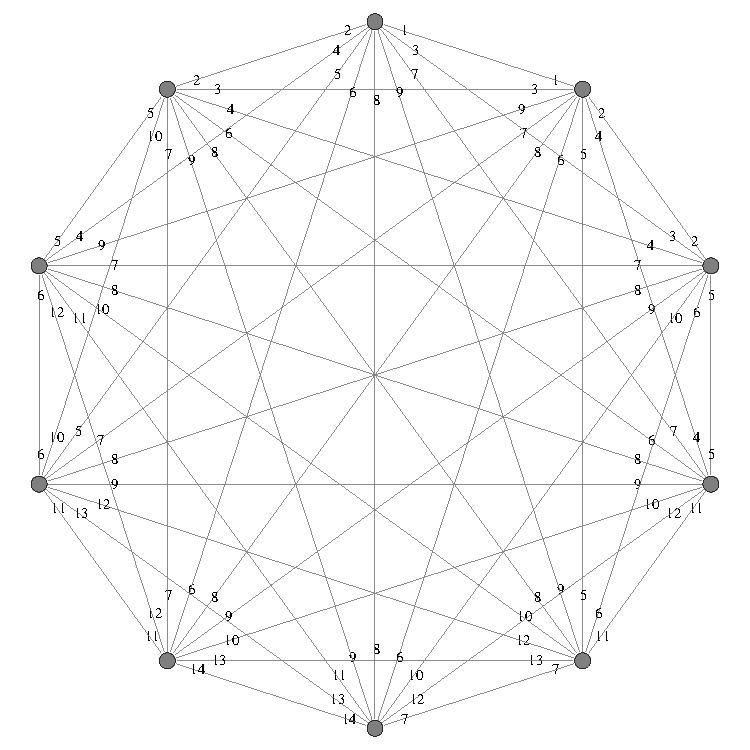
\includegraphics[width=0.74\textwidth]{figures/K_10-14.pdf}
\caption{$K_{10}$-ի միջակայքային $14$-ներկում: $sp(\alpha) = (1,2,1,1)$}
\label{t2_K10}
\end{figure}
\end{hide}

$W(K_{2n})$-ի հայտնի լավագույն վերին գնահատականը ստացել էին Գիառոն, Կուբալը և Մալաֆիյսկին. 
$W(K_{2n}) \leq 4n-4$, երբ $n \geq 2$:

\begin{hide}
\begin{hypothesis}
\label{h1_complete_log}
$W(K_{2n}) = 4n-2-\left \lfloor \log_2{n} \right \rfloor - \left \| n_2 \right \|$, որտեղ $\left \| n_2 \right \|$-ը $n$ թվի երկուական ներկայացման մեջ $1$-երի քանակն է:
\end{hypothesis}
\end{hide}
\begin{figure}[h]
\centering
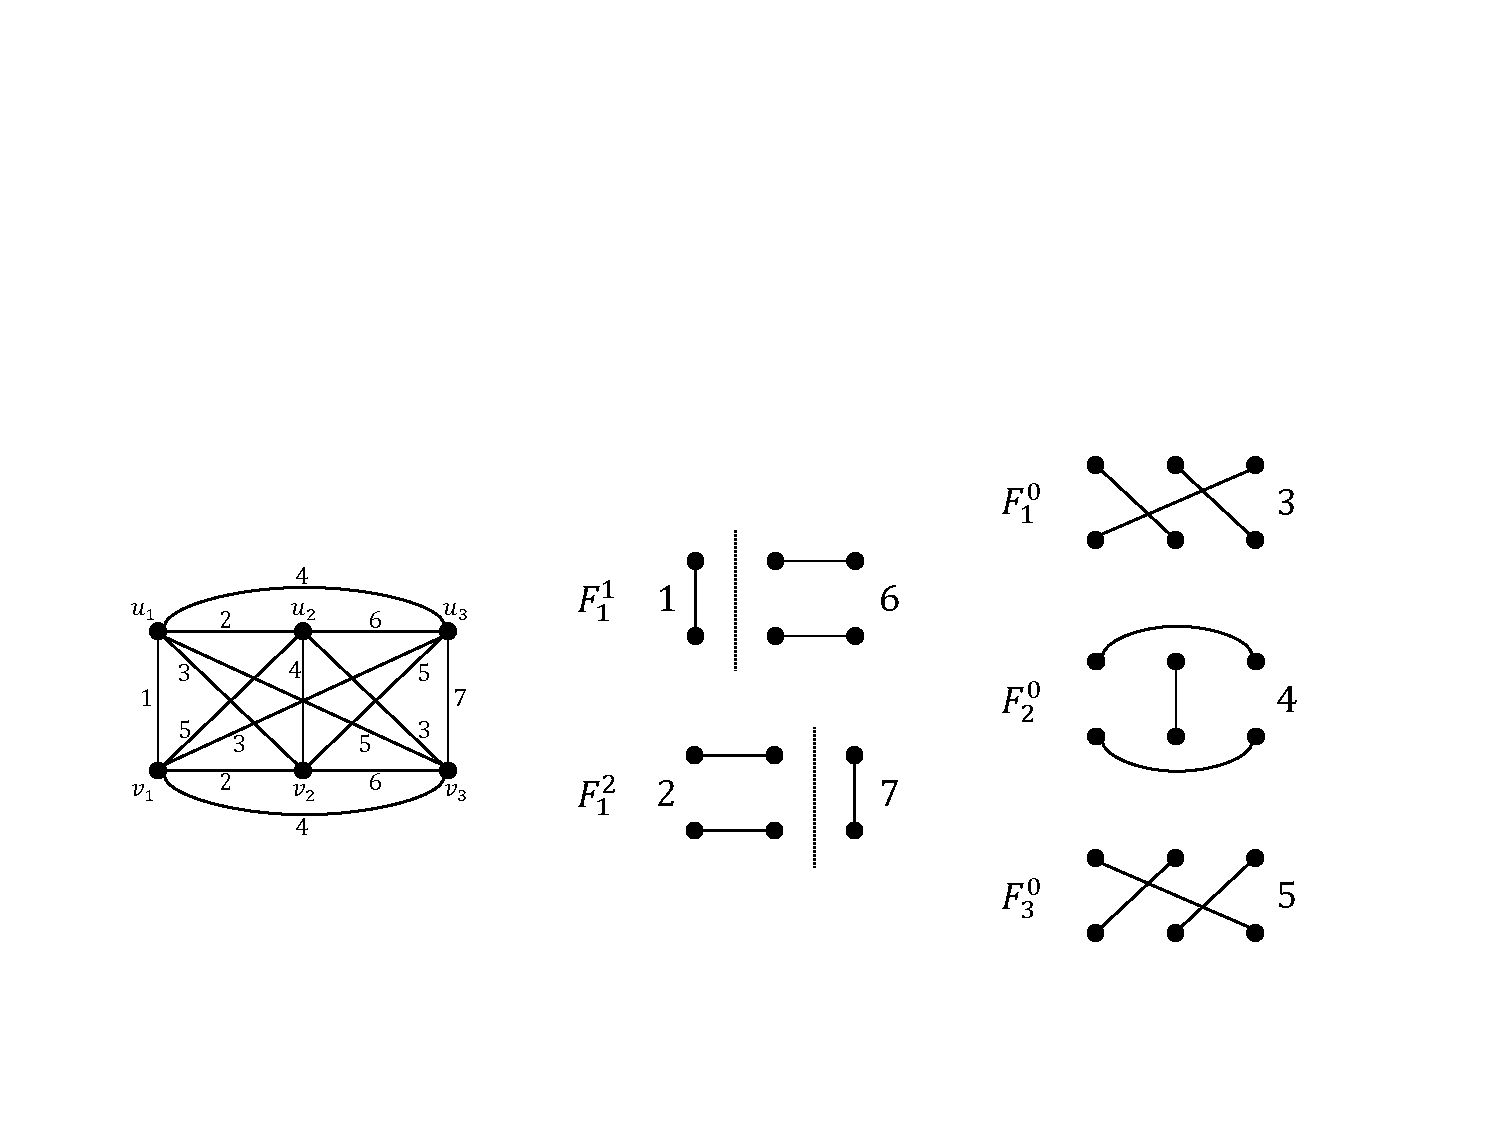
\includegraphics[width=0.7\textwidth]{figures/K_6factorization.pdf}
\caption{$K_6$-ի միջակայքային $7$-ներկումը և համապատասխան $1$-ֆակտորիզացիան՝ $\mathfrak{F}=\left\{F_1^1, F_1^2, F_1^0, F_2^0, F_3^0\right\}$}
\label{K_6factorization}
\end{figure}

$K_{2n}$ լրիվ գրաֆի գագաթների կամայական ֆիքսված $\mathbf{v} = \left(u_1,v_1, u_2,v_2, \ldots,u_n,v_n\right)$ համարակալման համար $H_{\mathbf{v}}^{[i,j]}$-ով, $i \leq j$, նշանակենք $K_{2n}$-ի $u_i, v_i, u_{i+1}, v_{i+1}, \ldots, u_j, v_j$ գագաթներով ծնված ենթագրաֆը: 

Դիցուք $\mathfrak{F} = \{F_1, F_2, \ldots, F_{2n-1}\}$ բազմությունը $K_{2n}$-ի $1$-ֆակտորիզացիա է: Ցանկացած $F\in \mathfrak{F}$ զուգակցման համար սահմանվում են իր \textit{ձախ և աջ մասերը} գագաթների $\mathbf{v}$ համարակալման նկատմամբ՝
\begin{center}
$l_{\mathbf{v}}^i(F) = F \cap E\left(H_{\mathbf{v}}^{[1,i]}\right)$ և
$r_{\mathbf{v}}^i(F) = F \cap E\left(H_{\mathbf{v}}^{[i+1,n]}\right)$:
\end{center}
Եթե որևէ $i$ թվի համար, $1 \leq i \leq n-1$, $F = l_{\mathbf{v}}^i(F) \cup r_{\mathbf{v}}^i(F)$, ապա $F$-ը կոչվում է \textit{$i$-բաժանված} կատարյալ զուգակցում $\mathbf{v}$ համարակալման նկատմամբ (օրինակ՝ $F_1^1$ և $F_1^2$ կատարյալ զուգակցումները Նկ. \ref{K_6factorization}-ում): Մի շարք լեմմաների օգնությամբ հաջողվել է ապացուցել լրիվ գրաֆի բաժանված կատարյալ զուգակցումներով ֆակտորիզացիաների և միջակայքային ներկումների համարժեքության լեմմա, որից բխում է հետևյալ արդյունքը.


\begin{hide}
\begin{remark}
\label{spectrumIntersection}
$K_{2n}$-ի ցանկացած $\alpha$ միջակայքային կողային ներկման համար, $S_\cap\left(K_{2n}, \alpha\right) \neq \emptyset$: Հակառակ դեպքում դա կհակասեր Թեորեմ \ref{t1_upper_2V-3}-ի վերին գնահատականին:
\end{remark}

\begin{lemma}
Եթե $1 \leq i \leq n$, ապա $\underline{S}(u_i, \alpha) = \underline{S}(v_i, \alpha)$.
\end{lemma}
\begin{proof}[Ապացույց]
Պնդում \ref{spectrumIntersection}-ից հետևում է, որ եթե $\underline{S}(v_i, \alpha) - \underline{S}(u_{i}, \alpha) > 0$, ապա $\underline{S}(u_{i}, \alpha)$ գույնով ներկված կողերը կազմում են կատարյալ զուգակցում $K_{2n}\left[\{u_1,v_1,u_2,v_2,\ldots,u_i\}\right]$ ենթագրաֆում, ինչը հնարավոր չէ, քանի որ այն ունի կենտ թվով գագաթներ:
\end{proof}

\begin{remark}
\label{totalShift}
Եթե $\alpha$-ն $K_{2n}$-ի միջակայքային $t$-ներկում է և ${\rm sh}(\alpha) = (b_1, b_2, \ldots, b_{n-1})$, ապա $t = 2n-1 + |{\rm sh}(\alpha)|$:
\end{remark}

\begin{remark}
\label{middleColors}
$K_{2n}$-ի կամայական $\alpha$ միջակայքային կողային ներկման համար բոլոր գագաթներում հանդիպող գույներն են. $S_\cap\left(K_{2n}, \alpha\right) = \left[\underline{S}(u_n, \alpha), \overline{S}(u_1, \alpha)\right] = \left[|{\rm sh}(\alpha)|+1, 2n-1\right] = \left\{|{\rm sh}(\alpha)|+j  : j=1,2,\ldots,2n-1-|{\rm sh}(\alpha)|\right\}$:
\end{remark}

\begin{remark}
\label{splittedColors}
Եթե $\alpha$-ն $K_{2n}$-ի միջակայքային $t$-ներկում է, և ${\rm sh}(\alpha) = (b_1, b_2, \ldots, b_{n-1})$, ապա
\begin{center}
\begin{tabular}{ll}
$L_{\mathbf{v}_\alpha}^i(\alpha) \subset S_\cap\left(H_{\mathbf{v}_\alpha}^{[1,i]},\alpha\right)$
&$L_{\mathbf{v}_\alpha}^i(\alpha) \cap S_\cup\left(H_{\mathbf{v}_\alpha}^{[i+1,n]},\alpha\right) = \emptyset$\\
$R_{\mathbf{v}_\alpha}^i(\alpha) \cap S_\cup\left(H_{\mathbf{v}_\alpha}^{[1,i]},\alpha\right) = \emptyset$ 
&$R_{\mathbf{v}_\alpha}^i(\alpha) \subset S_\cap\left(H_{\mathbf{v}_\alpha}^{[i+1,n]},\alpha\right)$
\end{tabular}
\end{center}
\end{remark}
\end{hide}

\begin{hide}
\begin{lemma}[Համարժեքության լեմմա]\label{lEquiv}
Հետևյալ երկու պնդումները համարժեք են.
\begin{description}
\item{(ա)} գոյություն ունի $K_{2n}$-ի $\alpha$ միջակայքային կողային ներկում այնպես, որ ${\rm sh}(\alpha) = (b_1, b_2, \ldots b_{n-1})$,
\item{(բ)} գոյություն ունի գագաթների $\mathbf{v}$ համարակալում և $K_{2n}$-ի $\mathfrak{F} = 
\left\{ F^0_j : j=1,2,\ldots,2n-1-\sum\limits_{i=1}^{n-1}b_i \right\}
\cup
\bigcup\limits_{i=1}^{n-1}\left\{F^i_j : j=1,2,\ldots,b_i\right\}$ $1$-ֆակտորիզացիա այնպես, որ $F^i_j$-ն $i$-բաժանված է $\mathbf{v}$ համարակալման նկատմամբ, $i=1,2,\ldots,n-1$, $j=1,2,\ldots,b_i$, $b_i \in \mathbb{Z}_+$:
\end{description}
\end{lemma}

\begin{proof}[Ապացույց]
Ապացույցի ընթացքում $B_i$-ով կնշանակենք $\sum\limits_{j=1}^{i}b_j$ գումարը, $i=0,1,\ldots,n-1$:

\begin{description}
\item{(ա) $=>$ (բ)}. Դիցուք $\alpha$-ն $K_{2n}$-ի միջակայքային $t$-ներկում է, որի համար ${\rm sh}(\alpha) = (b_1, b_2, \ldots b_{n-1})$: Ֆիքսենք գագաթների $\mathbf{v}_\alpha$ համարակալումը և կառուցենք $K_{2n}$-ի $\mathfrak{F}$ $1$-ֆակտորիզացիան: 

Պնդում \ref{middleColors}-ի համաձայն գոյություն ունեն $2n-1-|{\rm sh}(\alpha)|$ գույներ, որոնք հանդիպում են բոլոր գագաթների սպեկտրներում: Ըստ սահմանման, $|{\rm sh}(\alpha)| = \sum\limits_{i=1}^{n-1}b_i$, ուստի կարող ենք վերցնել $F_j^0 = C_{|{\rm sh}(\alpha)|+j}(\alpha)$, որտեղ $j=1,2,\ldots,2n-1-|{\rm sh}(\alpha)|$:

Պնդում \ref{splittedColors}-ից հետևում է, որ ցանկացած $i=1,2,\ldots,n-1$, թվի համար գոյություն ունեն $|L_{\mathbf{v}_\alpha}^i(\alpha)|=b_i$ իրարից տարբեր գույներ, որոնք հանդիպում են միայն գագաթների առաջին $i$ զույգերի սպեկտրներում, և ևս $|R_{\mathbf{v}_\alpha}^i(\alpha)|=b_i$ իրարից տարբեր գույներ, որոնք հանդիպում են միայն մնացած $2n-2i$ գագաթների սպեկտներում: Վերցնենք $F^i_j = C_{B_{i-1} + j}(\alpha) \cup C_{B_{i-1} + 2n - 1 + j}(\alpha)$, կամայական $i=1,2,\ldots,n-1$ և $j=1,2,\ldots,b_i$ թվերի համար: Նկատենք, որ $L_{\mathbf{v}_\alpha}^i(\alpha) \cup R_{\mathbf{v}_\alpha}^i(\alpha)$ բազմության գույներով ներկված կողերը չեն հատում $i$-րդ և $(i+1)$-րդ գագաթների զույգերի միջև անցնող ուղղահայաց ուղիղը ($F_1^1$ և $F_1^2$ Նկ. \ref{K_6factorization}-ում), ուստի $F^i_j$-ն բոլոր թույլատրելի $j$-երի համար $i$-բաժանված կատարյալ զուգակցում է գագաթների $\mathbf{v}_\alpha$ համարակալման նկատմամբ:

\item{(բ) $=>$ (ա)}. Ենթադրենք $\mathfrak{F} = 
\left\{ F^0_j : j=1,2,\ldots,2n-1-|{\rm sh}(\alpha)| \right\}
\cup
\bigcup\limits_{i=1}^{n-1}\left\{F^i_j : j=1,2,\ldots,b_i\right\}$ $K_{2n}$-ի $1$-ֆակտորիզացիա է, ընդ որում $F_j^i$-ն $i$-բաժանված կատարյալ զուգակցում է գագաթների $\mathbf{v}=\left(u_1,v_1, u_2,v_2, \ldots,u_n,v_n\right)$ համարակալման նկատմամբ, $i=1,2,\ldots,n-1$, $j=1,2,\ldots,b_i$: Կառուցենք $K_{2n}$-ի $\alpha$ միջակայքային կողային ներկումը հետևյալ կերպ.

\begin{tabular}{lll}
$\alpha(e)=B_{i-1} + j$ & երբ $e \in l_{\mathbf{v}}^i(F_j^i)$ & $i=1,2,\ldots,n-1$, $j=1,2,\ldots,b_i$ \\
$\alpha(e)=B_{n-1} + j$ & երբ $e \in F_j^0$ & $j=1,2,\ldots,2n-1-B_{n-1}$\\
$\alpha(e)=B_{i-1} + 2n - 1 + j$ & երբ $e \in r_{\mathbf{v}}^i(F_j^i)$ & $i=1,2,\ldots,n-1$, $j=1,2,\ldots,b_i$
\end{tabular}

Այն փաստից, որ $F^i_j$-ն գագաթների $\mathbf{v}$ համարակալման նկատմամբ $i$-բաժանված կատարյալ զուգակցում է, հետևում է, որ $K_{2n}$-ի կամայական կող ստացել է որևէ գույն: Իրոք, $u_i$ (նաև $v_i$) գագաթը ծածկված է բոլոր $F_j^0$ զուգակցումներով, $j=1,2,\ldots,2n-1-B_{n-1}$, $F_j^{i'}$, զուգակցումների ձախ մասերով, $i'=i,i+1,\ldots,n-1$, և $F_j^{i'}$ զուգակցումների աջ մասերով, $i'=1,2,\ldots,i-1$, կամայական $j=1,2,\ldots,b_{i'}$ թվի համար: Ուստի գագաթների սպեկտրները կլինեն.
\begin{align*}
S(u_i, \alpha) = S(v_i, \alpha) &= \bigcup\limits_{i'=i}^{n-1}\{B_{i'-1} + j  : j=1,2,\ldots,b_{i'}\} \\
& \cup
\{B_{n-1} + j : j=1,2,\ldots,2n-1-B_{n-1}\} \\
& \cup
\bigcup\limits_{i'=1}^{i-1}\{B_{i'-1} + 2n-1 + j  : j=1,2,\ldots,b_{i'}\}\\
&= [B_{i-1}+1, B_{n-1}] \cup [B_{n-1}+1, 2n-1] \cup [2n, B_{i-1}+2n-1]\\
&= [B_{i-1}+1, B_{i-1}+2n-1]
\end{align*}

Սա ցույց է տալիս, որ $\alpha$-ն $K_{2n}$-ի  միջակայքային $(B_{n-1} + 2n-1)$-ներկում է: Լեմմայի ապացույցն ավարտելու համար անհրաժեշտ է ստուգել կառուցված $\alpha$ ներկման շեղումների վեկտորը: Նկատենք, որ կամայական $i=1,2,\ldots,n-1$, թվի համար ունենք, որ $\underline{S}(u_{i+1}, \alpha) - \underline{S}(u_{i}, \alpha) = B_{i}-B_{i-1} = b_i$: Սա նշանակում է, որ գագաթների $\mathbf{v}_\alpha$ համարակալումը համընկնում է $\mathbf{v}$ համարակալման հետ և ${\rm sh}(\alpha) = (b_1, b_2, \ldots, b_{n-1})$:
\end{description}

\end{proof}

\begin{remark}\label{splittedSameColor}
Համարժեքության լեմմայի ապացույցի առաջին մասում կառուցված $F_j^0$ զուգակցումների մի մասը ևս կարող են լինել բաժանված կատարյալ զուգակցումներ, սակայն նրանց թե՛ աջ և թե՛ ձախ մասերը $\alpha$ ներկման մեջ ունեն նույն գույնը: Օրինակ, երբ $|{\rm sh}(\alpha)|=0$, $F^0_{\alpha(u_1v_1)} = C_{\alpha(u_1v_1)}(\alpha)$ զուգակցումը $1$-բաժանված կատարյալ զուգակցում է գագաթների $\mathbf{v}_\alpha$ համարակալման նկատմամբ:
\end{remark}
\end{hide}

\begin{corollary}\label{cEquiv}
Ցանկացած $n\in\mathbb{N}$-ի համար $K_{2n}$-ը ունի միջակայքային $t$-ներկում այն և միայն այն դեպքում, երբ այն ունի այնպիսի $1$-ֆակտորիզացիա, որտեղ առնվազն $t-2n+1$ կատարյալ զուգակցումներ բաժանված են:
\end{corollary}
\begin{proof}[Ապացույց]
Տրված միջակայքային $t$-ներկմանը համապատասխանող $1$-ֆակտորիզացիայի կառուցումը անմիջականորեն հետևում է Պնդում \ref{totalShift}-ից և Համարժեքության լեմմայից: Պնդում \ref{splittedSameColor}-ից հետևում է, որ ստացված $1$-ֆակտորիզացիայում բաժանված կատարյալ զուգակցումների թիվը կարող է մեծ լինել $t-2n+1$ թվից:

Եթե տրված է $K_{2n}$-ի $1$-ֆակտորիզացիա, որտեղ առնվազն $t-2n+1$ կատարյալ զուգակցումներ բաժանված են, կարող ենք դրանցից ընտրել որևէ $t-2n+1$-ը, ապա դրանցից յուրաքանչյուրի համար ընտրել որևէ $i$ թիվ, որի համար այն $i$-բաժանված է (միևնույն կատարյալ զուգակցումը կարող է միաժամանակ լինել և՛ $i$-բաժանված, և՛ $i'$-բաժանված տարբեր $i$ և $i'$ թվերի համար, ընտրությունը կրկին կամայական է) և կիրառել Համարժեքության լեմման: Այսպիսով, ստացված ներկումը կարող է միակը չլինել:
\end{proof}

Այս հետևանքի հիման վրա 1.4 ենթագլխում ապացուցվել են $W(K_{2n})$-ի մի շարք նոր ստորին և վերին գնահատականներ: